\documentclass[10pt, a4paper]{article}

%%% SST LAB PROTOCOLL PREAMBLE
%%% 2019
%%%%%%%%%%%%%%%%%%%%%%%%%%%%%%%


%%% PACKAGES
%%%%%%%%%%%%%%%%%%%%%%%%%%%

\usepackage[ngerman]{babel}

\usepackage[utf8]{inputenc}
\usepackage{amsmath}
\usepackage{pgfplots}
\usepackage{tikz}
\usepackage[many]{tcolorbox}
\usepackage{graphicx}
\graphicspath{ {./graphics/} }
\usepackage{pdfpages}
\usepackage{dashrule}
\usepackage{float}
\usepackage{siunitx}
\usepackage{trfsigns}
\usepackage{booktabs}
\usepackage[european]{circuitikz}
\usepackage{tcolorbox}

%%% DOCUMENT GEOMETRY
%%%%%%%%%%%%%%%%%%%%%%%%%%%

\usepackage{geometry}
\geometry{
 a4paper,
 total={0.6180339887498948\paperwidth,0.6180339887498948\paperheight},
 top = 0.1458980337503154\paperheight,
 bottom = 0.1458980337503154\paperheight
 }
\setlength{\jot}{0.013155617496424828\paperheight}
\linespread{1.1458980337503154}

\setlength{\parskip}{0.013155617496424828\paperheight} % paragraph spacing


%%% COLORS
%%%%%%%%%%%%%%%%%%%%%%%%%%%

\definecolor{red1}{HTML}{f38181}
\definecolor{yellow1}{HTML}{fce38a}
\definecolor{green1}{HTML}{95e1d3}
\definecolor{blue1}{HTML}{66bfbf}
\definecolor{hsblue}{HTML}{00b1db}
\definecolor{hsgrey}{HTML}{afafaf}

%%% CONSTANTS
%%%%%%%%%%%%%%%%%%%%%%%%%%%
\newlength{\smallvert}
\setlength{\smallvert}{0.0131556\paperheight}


%%% COMMANDS
%%%%%%%%%%%%%%%%%%%%%%%%%%%

% differential d
\newcommand*\dif{\mathop{}\!\mathrm{d}}

% horizontal line
\newcommand{\holine}[1]{
  	\begin{center}
	  	\noindent{\color{hsgrey}\hdashrule[0ex]{#1}{1pt}{3mm}}\\%[0.0131556\paperheight]
  	\end{center}
}

% mini section
\newcommand{\minisec}[1]{ \noindent\underline{\textit {#1} } \\}

% quick function plot
\newcommand{\plotfun}[3]{
  \vspace{0.021286\paperheight}
  \begin{center}
    \begin{tikzpicture}
      \begin{axis}[
        axis x line=center,
        axis y line=center,
        ]
        \addplot[draw=red1][domain=#2:#3]{#1};
      \end{axis}
    \end{tikzpicture}
  \end{center}
}

% box for notes
\newcommand{\notebox}[1]{

\tcbset{colback=white,colframe=green1!100!black,title=Note!,width=0.618\paperwidth,arc=0pt}

 \begin{center}
  \begin{tcolorbox}[]
   #1 
  \end{tcolorbox}
 
 \end{center} 
 
}

% box for equation
\newcommand{\eqbox}[2]{
	
	\tcbset{colback=white,colframe=green1!100!black,title=,width=#2,arc=0pt}
	
	\begin{center}
		\begin{tcolorbox}[ams align*]
				#1
		\end{tcolorbox}
		
	\end{center} 
	
}
% END OF PREAMBLE

\newtcbox{\inlinecodee}{on line, boxrule=0pt, boxsep=0pt, top=2pt, left=2pt, bottom=2pt, right=2pt, colback=gray-2, colframe=white, fontupper={\ttfamily \footnotesize}}


\addbibresource{sources.bib}

\begin{document}


\includepdf{./titlepage/titlepage.pdf}

\section{Introduction}
The DFT/FFT is acting on discrete sequences which usually come from some form of finite-time real world measurement. Even if the sample rate is suffient enough as to not cause aliasing, signal frequency content that lies in between DFT frequency bins (i.e. not exactly at a multiple of $\Delta f = \frac{f_{\text{sample}}}{N}$) will cause so-called \textit{spectral leakage}. This means that the energy will be spread to the adjacent bins of the actual signal frequency.
\\

This can be understood by thinking of a sinusoidal signal being cut out by a rectangular window that is a sequence of all ones inside the sampling interval and zeros outside. This cutting-out happens by multiplication, meaning that in frequency domain, it will be the convolution of the signal's spectrum with the rectangular spectrum which is a sinc function. Now, the FFT will sample this continuous spectrum in steps of $\Delta f = \frac{f_{\text{sample}}}{N}$. If the input frequency is not a multiple of this then the values around the nearest multiple (as well as further ones) will be those of the window's sinc function. Figure \ref{fig:intro1} illustrates this.\\%\footnote{The representation is not fully accurate, as there might be higher leakage values on the left due to ``wrapping'' from the negative frequency side, see \cite{understanding_dsp}.}.\\

\begin{figure}[h]
  \centering
  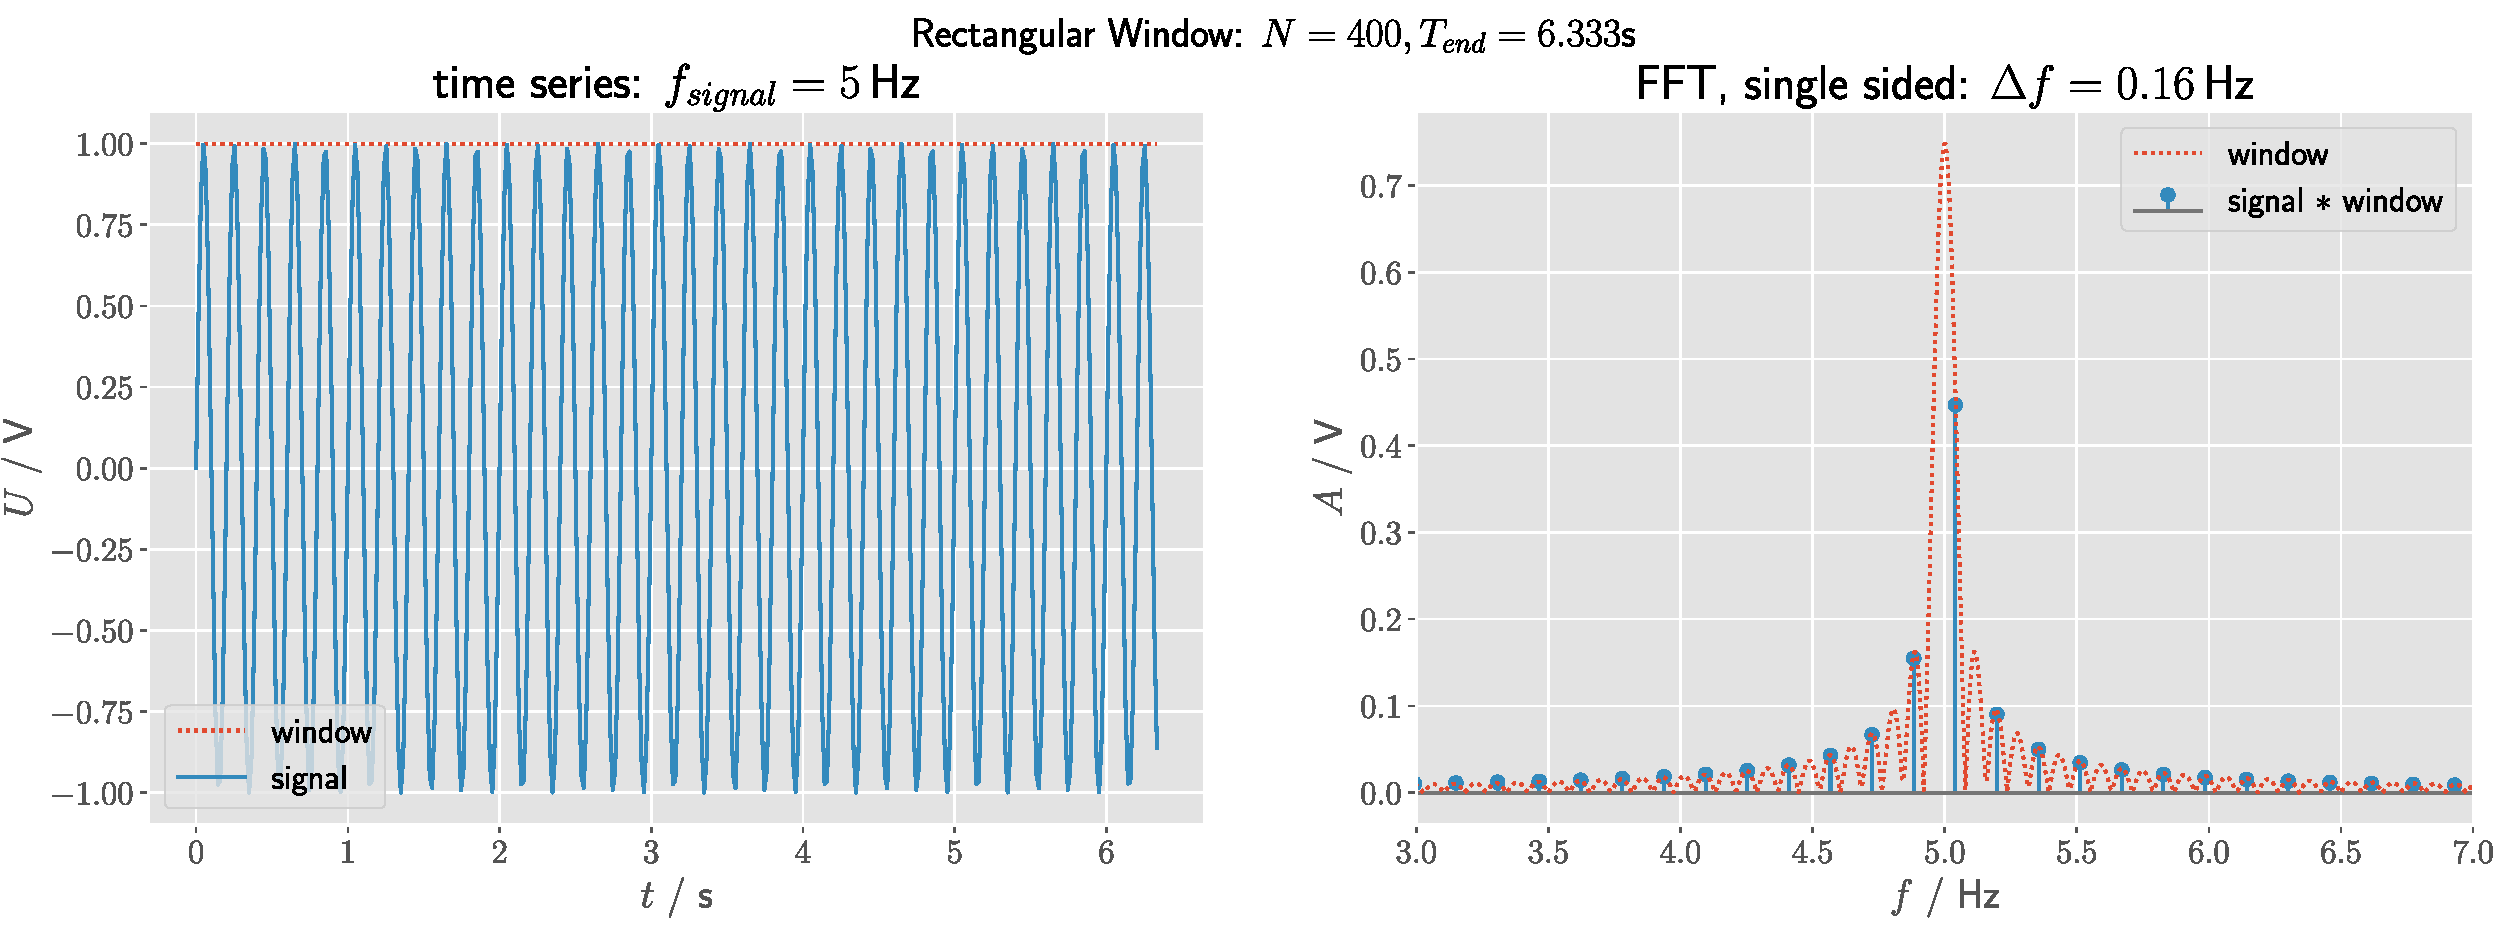
\includegraphics[width=\textwidth]{graphics/intro.pdf}
  \caption{Visualization of DFT spectral leakage. Note the discontinuity from the last to the first sample in the time series.}\label{fig:intro1}
\end{figure}


One obvious way to reduce the leakage is to increase the sample interval (enlargen the rectangular window) which in turn reduces the width of the convoluting sinc function as well as the frequency domain resolution.
Another way is to change the shape of the window by applying a windowing function to the time domain sequence. This aims to bring the samples at the beginning and end of the sequence towards a common value, thereby reducing any discontinuity (i.e. you can periodically continue the sequence without any ``jumps''). \cite{understanding_dsp}\\

The following will investigate the influence of different windowing functions using python with \inlinecodee{scipy}, \inlinecodee{numpy}, and \inlinecodee{matplotlib}. The full python script can be found in appendix \ref{app:script}.

\section{Signal under Test}
The number of points has been chosen to be $N=600$. With a total time window of $T=2\,\si{\second}$ this results in a sampling frequency of $f_{\text{s}} = \frac{N}{T} = 300\,\si{\hertz}$ and an FFT frequency step size of $\Delta f = \frac{1}{T} = 0.5\,\si{\hertz}$

The signal used in each case is a sum of three sinusoids:
\[
u(t) = 1\,\si{\volt} \cdot \sin{(2\pi f_{0} \cdot t)} + 1\,\si{\volt}\sin{(2\pi f_{1} \cdot t)} + 1\,\si{\volt}\sin{(2\pi f_{2} \cdot t)}
\]
with
\begin{align*}
  f_{0} &= 1.5\,\si{\hertz}\\
  f_{1} &= 4.25\,\si{\hertz}\\
  f_{2} &= 6.1\,\si{\hertz}
\end{align*}

The frequencies have been chosen such that one lies exactly on a multiple of $\Delta f$ ($f_{0}$), one exactly half way between two multiples ($f_{1}$), and one lies close to a multiple ($f_{2}$).

Figure \ref{fig:win_rect} shows the signal in time and its fft.


\section{Windowing Results}

\subsection{Rectangular}
In the time domain, there is a clear discontinuity between start and end of the time series and as expected, the spectral leakage is present in the spectrum (figure \ref{fig:win_rect}).
This spectrum will be used as a reference. The figures of the following window types will show their differences towards this reference window in their spectra for comparison.

\begin{figure}[h]
  \centering
  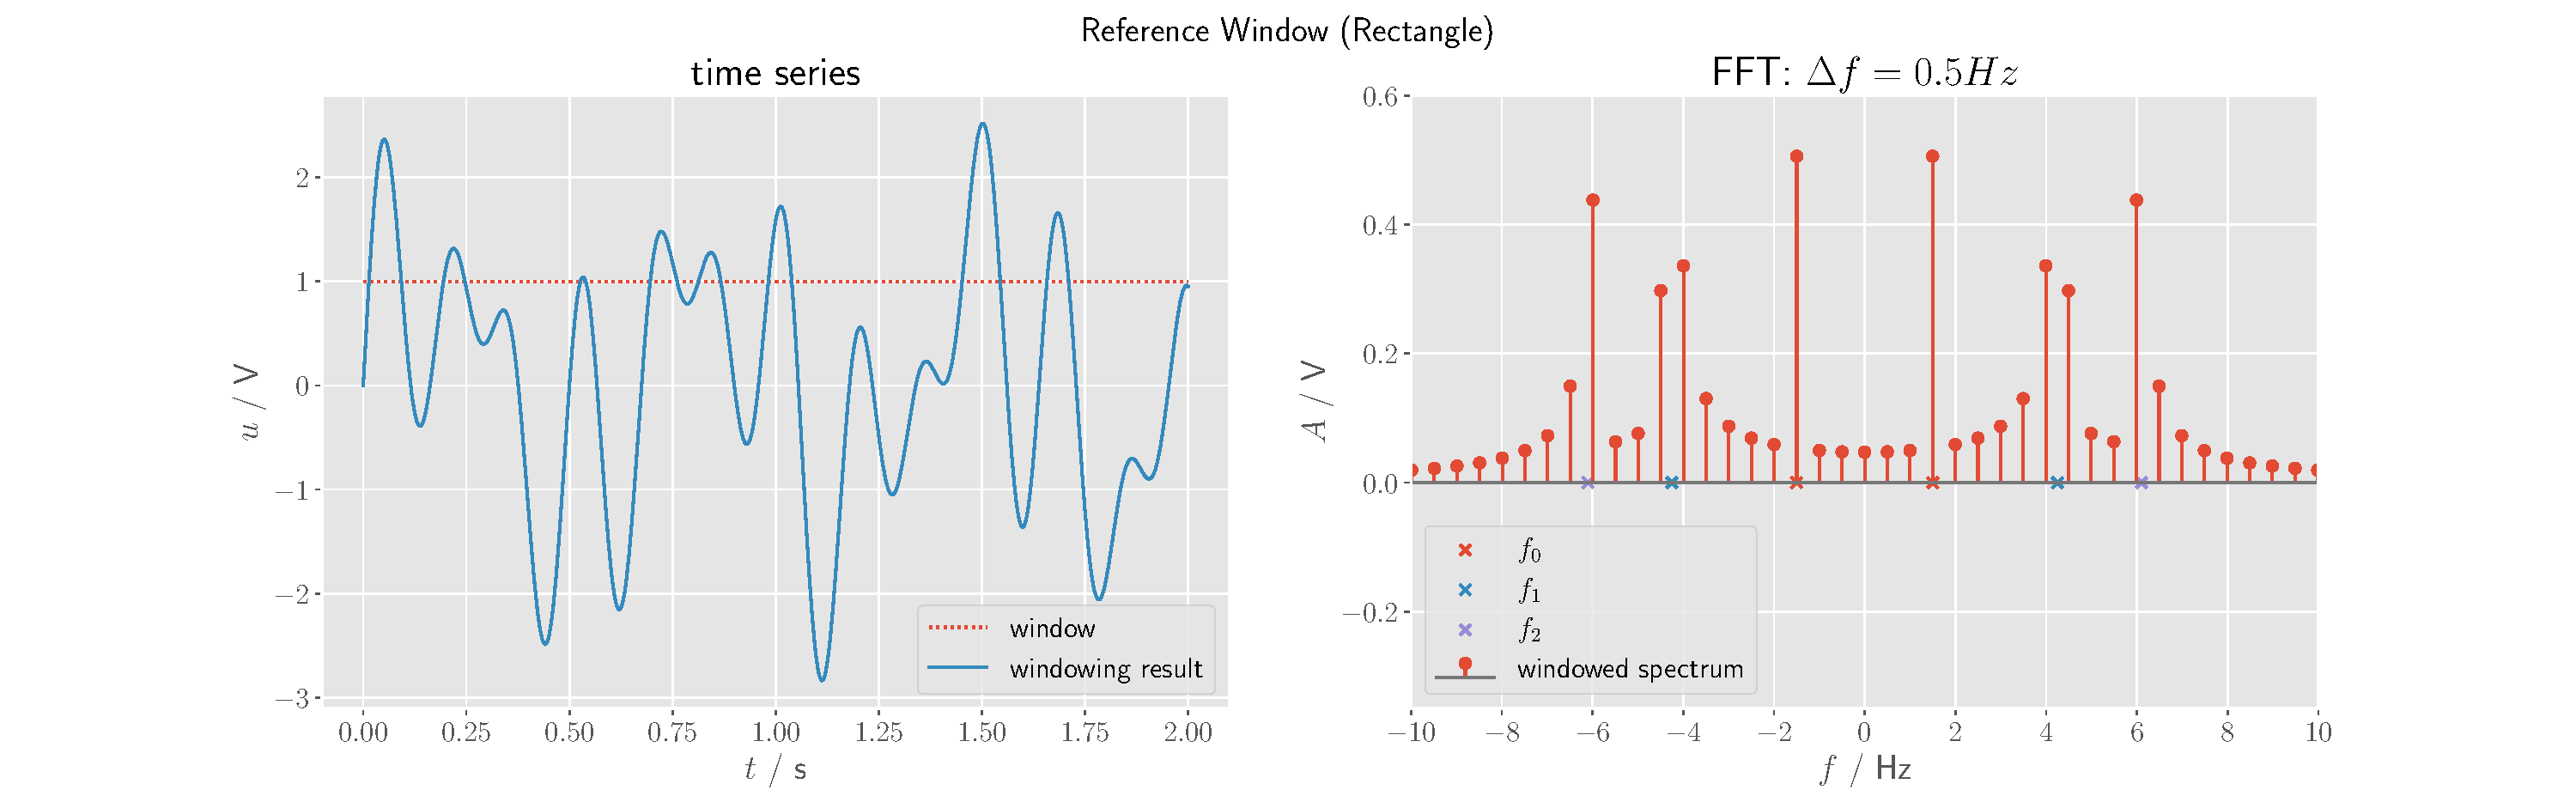
\includegraphics[width=\textwidth]{graphics/Rectangle.pdf}
  \caption{Time series and FFT with rectangular window (default).}\label{fig:win_rect}
\end{figure}

As for the signal frequencies, $f_{0}$ is exactly at a multiple of $\Delta f$ and does not seem to produce any leakage. $f_{1}$'s spectral content is approximately evenly split between the two adjacent bins. $f_{2}$'s split is in favour of the closer frequency bin.


\subsection{Bartlett}
The Bartlett window is a form of triangular window where the beginning and end points are zero. \cite{scipy_doc_bartlett} A triangular pulse/window also is of sinc-shape like the rectangular window, however it falls off more rapidly with frequency \cite{triang_pulse}\cite{ulrich_maths}, which makes it a potentially better candidate of a windowing function.


Figure \ref{fig:win_bartlett} shows the effective reduction of the leakage around the signal frequencies. The positive differences, however, indicate an increase in leakage, especially around $f_{0}$. This will be the case for all window types discussed here.

%Note: change freq to 3,4,5 and observe the wideness of the bartlett o boi??\\
%Note: change in NUM_ not affecting spectrum...


\subsection{Hanning}
The Hanning window has a shape that results in a time series quite similar to the Bartlett window (figure \ref{fig:win_hann}). The difference is best seen in the comparison of the window spectra as seen in figure \ref{fig:win_spec_comp}. The Bartlett window falls off rapidly with frequency but shows quite high side lobes which means it might be better suited for features that are closer in frequency. This behaviour can also be seen in figures \ref{fig:win_hann} and \ref{fig:win_bartlett}, e.g. at the samples around $f_{2}$.


\subsection{Hamming}
The hamming window shows a main lobe that is less wide than that of the hanning window but it does not drop off as fast for the higher side lobes. \cite{understanding_dsp} This is also to an extend visible in figure \ref{fig:win_hamm}. So, for frequency bins closer to the signal frequency, there will be less leakage than with the hanning window but it is the opposite for bins further away.


\begin{figure}[h]
  \centering
  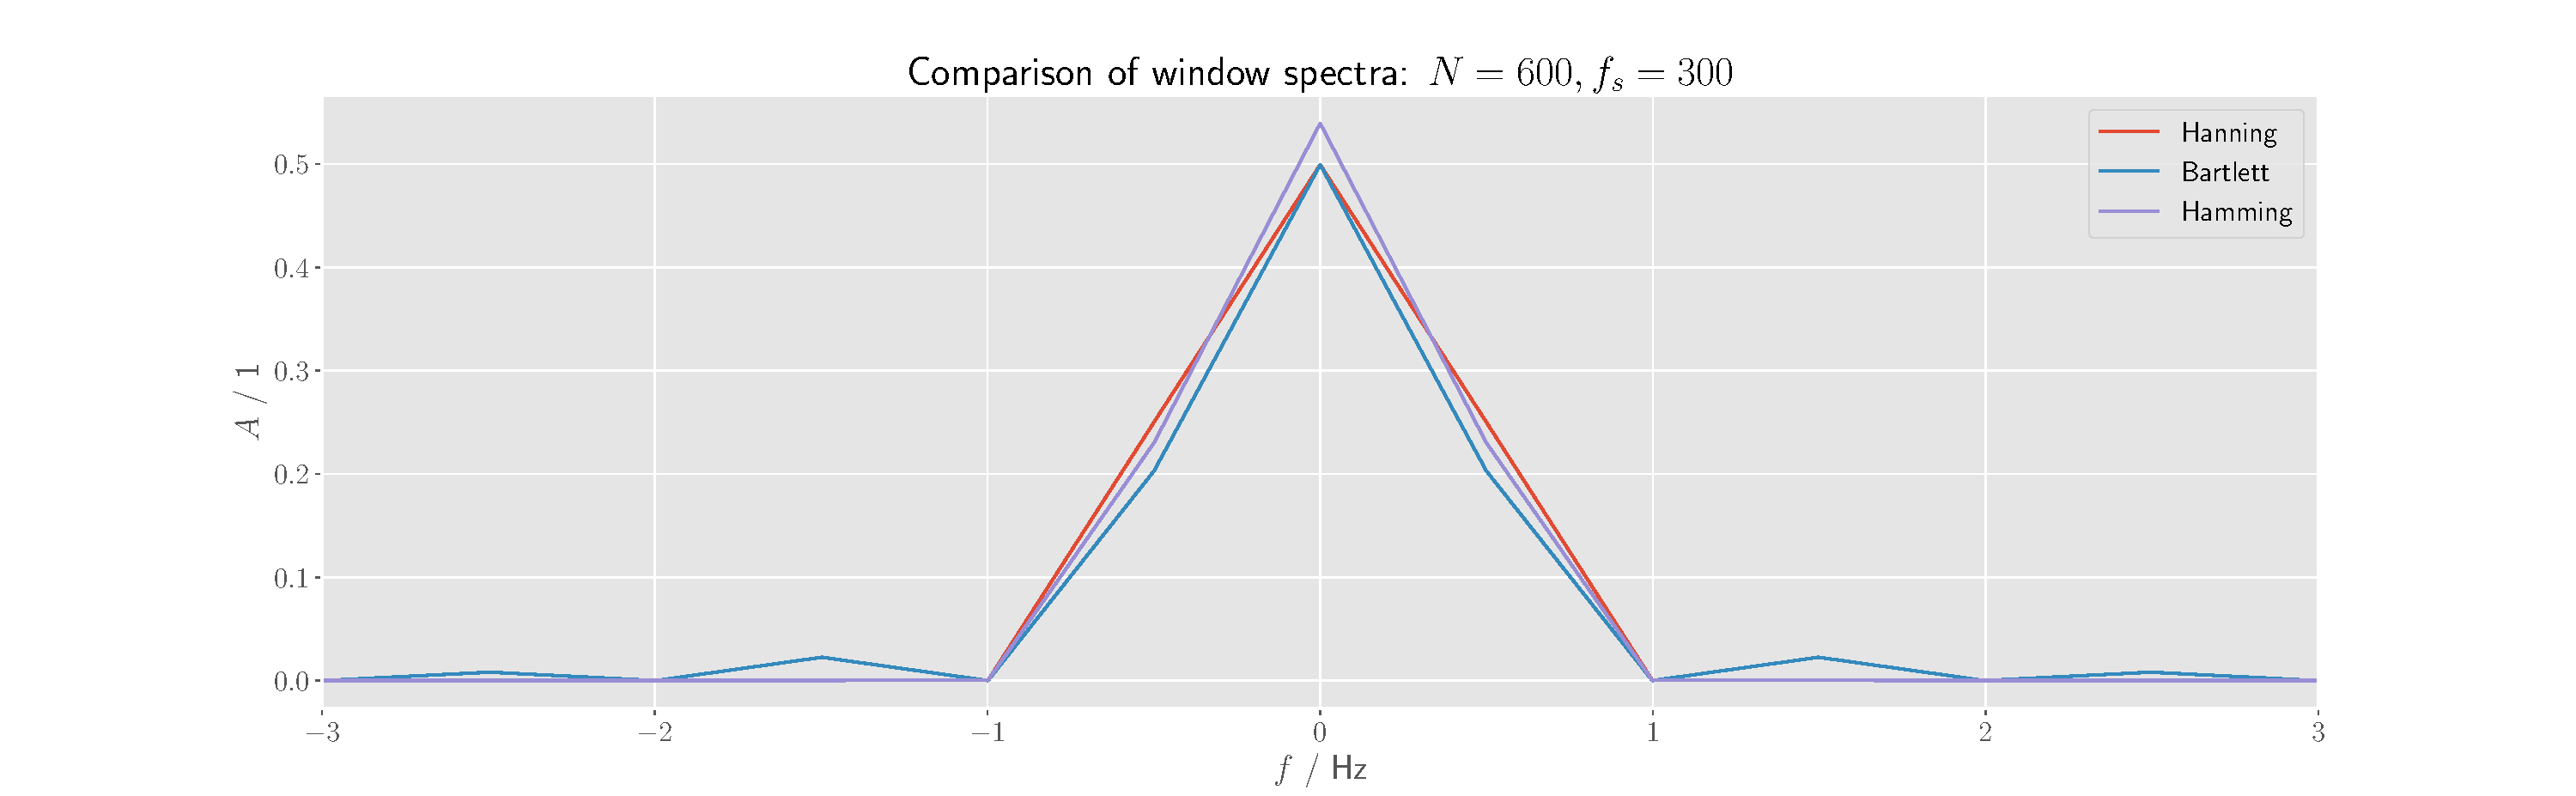
\includegraphics[width=\textwidth]{graphics/win_spectra.pdf}
  \caption{Comparison of the spectra of the used windows.}\label{fig:win_spec_comp}
\end{figure}

% \subsection{Gaussian}
% The fourier transform of a gaussian bell curve is also a gaussian. \cite{ulrich_maths} Since it extends to infinity, i.e. is not zero at the sampling interval edges, some discontinuities will remain. This means the standard deviation $\sigma$ has to be chosen carefully. On one hand, if it is too large the window's effect might not be sufficient. On the other hand, too small of a standard deviation will shrink great amounts of the time series and cause a wider spectrum. In this case, a standard deviation of $80$ samples has been chosen.

\begin{figure}[H]
  \centering
  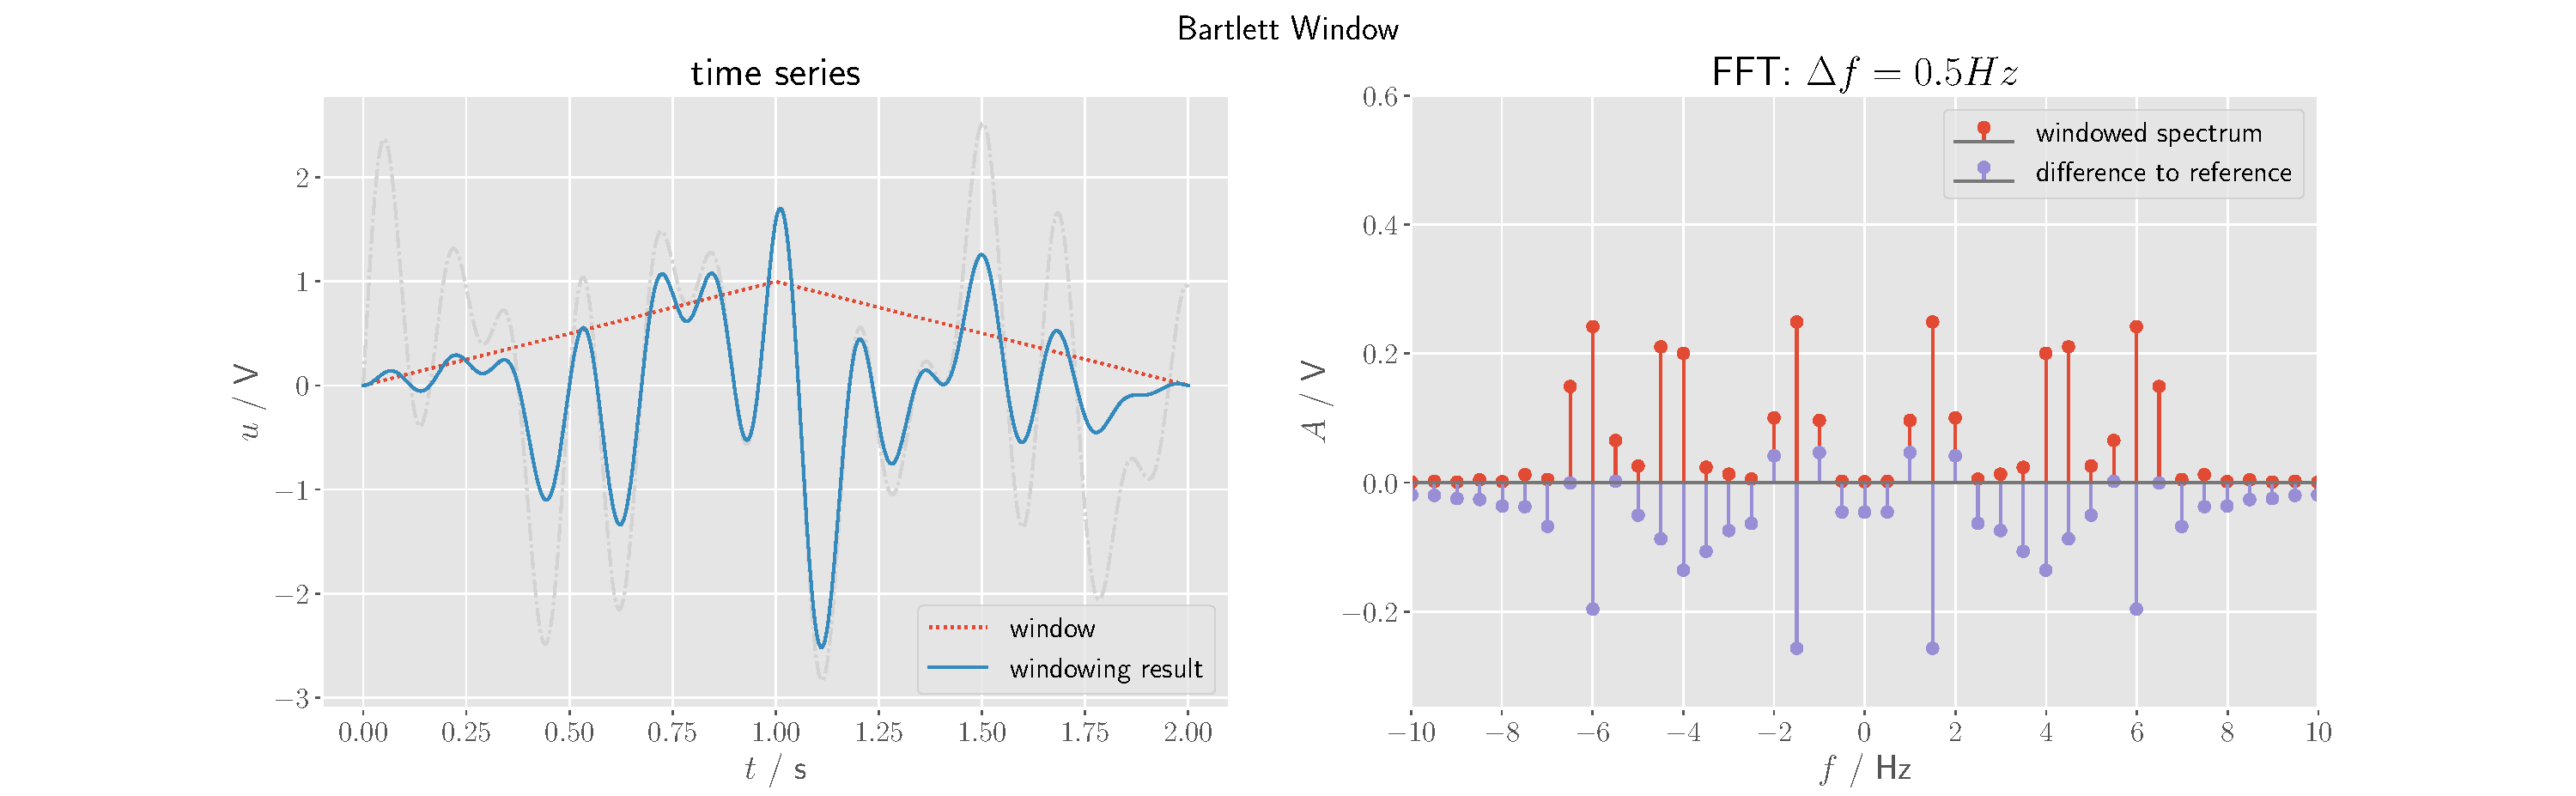
\includegraphics[width=\textwidth]{graphics/Bartlett.pdf}
  \caption{Time series and FFT after applying the Bartlett window.}\label{fig:win_bartlett}
\end{figure}


\begin{figure}[H]
  \centering
  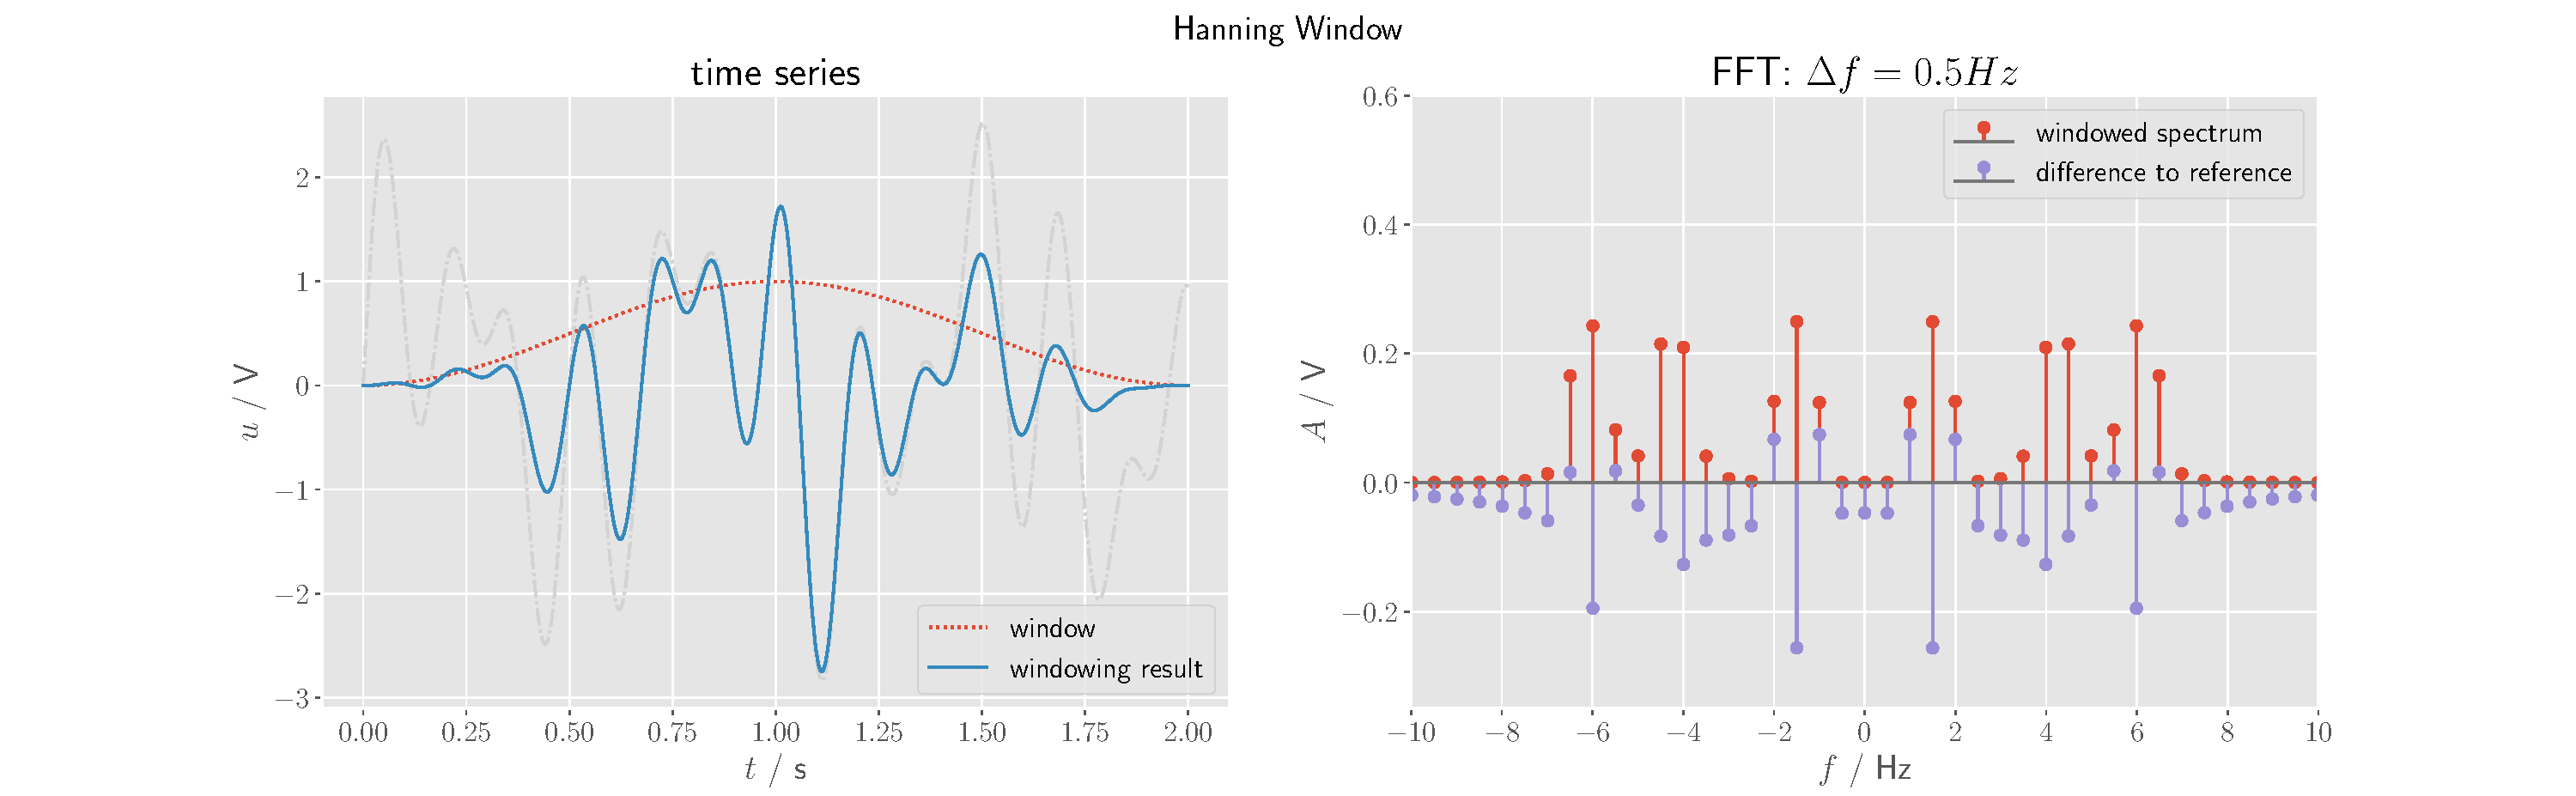
\includegraphics[width=\textwidth]{graphics/Hanning.pdf}
  \caption{Time series and FFT after applying the Hann window.}\label{fig:win_hann}
\end{figure}

\begin{figure}[H]
  \centering
  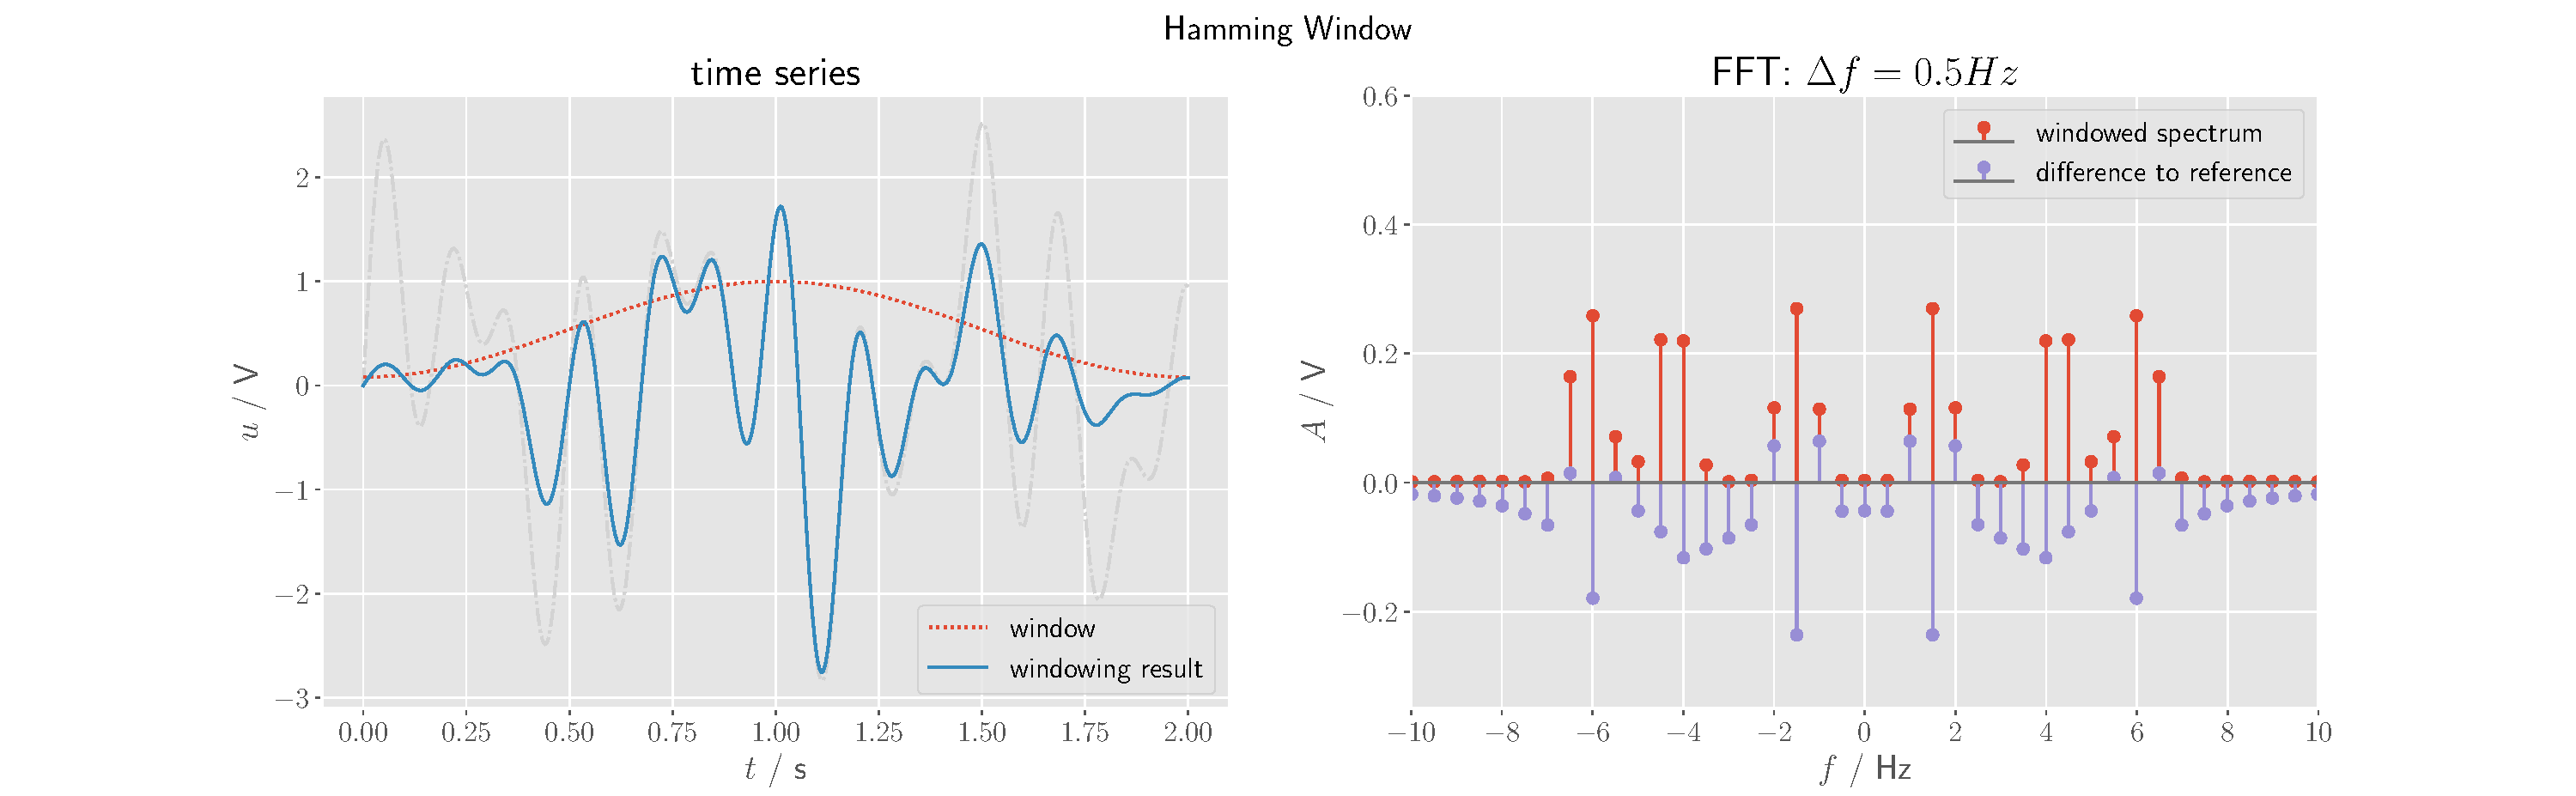
\includegraphics[width=\textwidth]{graphics/Hamming.pdf}
  \caption{Time series and spectrum after applying the Hamming window.}\label{fig:win_hamm}
\end{figure}


\section{Conclusion}
The difference between these three window types is not large in this example. However, all have in common that they reduce the spectral leakage of the rectangular window's spectral side lobes. %Also, each applied window brought the different spectral amplitudes (bins, resp.) of the signal's harmonics closer together, as is the case with the actual sinusoidal since they are $1\,\si{\volt}$ each. Wrong!

In each case, the amplitudes of the harmonic frequencies of interest were reduced as well. Each window function introduced a reduction by a factor of approximately $0.5$. Also, for frequencies that lie exactly on a multiple of $\Delta f$, windowing actually increases the leakage.
This means that in practice, the reduction of the main lobe in relation to the side lobes of the windows may have to be evaluated depending on the signal of interest.

\printbibheading

\begin{refsection}[sources.bib]
\nocite{*}
\printbibliography[heading=subbibliography,title={Literature}]
\end{refsection}

\begin{refsection}[software.bib]
\nocite{*}
\printbibliography[heading=subbibliography,title={Software Used}]
\end{refsection}

\pagebreak
\appendix
\section{Python Code}\label{app:script}

\lstinputlisting{./code/windowing.py}

\end{document}
